%
% Copyright (c) 2010 
% Manuel Vonthron - <manuel DOT vonthron AT acadis DOT org>
%
% This file may be distributed and/or modified under the terms of 
% the Do What The Fuck You Want To Public License, Version 2
% 

\documentclass{beamer}

\usepackage[french]{babel}
\usepackage{csquotes}
\usepackage{xcolor}
\usepackage{mdframed}

\definecolor{lightgray}{RGB}{150,150,150}
\definecolor{shadecolor}{RGB}{255,241,204}

\mdfdefinestyle{yellowbox}{%
    linecolor=white, linewidth=0pt,
    backgroundcolor=shadecolor,
    leftline=false, rightline=false,
    innertopmargin=0.25cm, innerbottommargin=0.25cm,
    innerleftmargin=0.25cm, innerrightmargin=0.25cm,
}

\usetheme[
        %url={nano.polymtl.ca},
        %numbering={false},
        menuwidth={0.3\paperwidth}
        ]{polymtl}

\setbeamercovered{transparent=20}

\begin{document}

\title[Présentation d'article INF6600]{How to address certification for multi-core based IMA platforms :
       current status and potential solutions} 
\subtitle{\vspace{1em} Présentation de l'article}
\author{ \vspace{2em} Antonin Godard} 
\date{\today} 
\institute{\'Ecole Polytechnique de Montr\'eal \\ 
  \vspace{-0.2em}{\small INF6600} }

\begin{frame}[plain]
  \titlepage
\end{frame}


\begin{frame}{Table of contents}
  \tableofcontents
\end{frame}


\section{Expliquons le titre…} 
\begin{frame}[t]{Multicore based IMA} 
  
  \begin{center}
    \begin{mdframed}[style=yellowbox]
      {\small\textcolor{lightgray}{How to address certification for} multi-core based IMA \textcolor{lightgray}{platforms :
       current status and potential solutions}}
       \end{mdframed}
  \end{center}
  
  \begin{itemize}
      \item De modules LRU à un AMI :
      \begin{itemize}
          \item \textit{Line Replacable Unit} : module d'un avion effectuant une fonction spécifique, et qui est \textbf{remplaçable} rapidement. \\
          \begin{center}
              $\downarrow$
          \end{center}
          \item \textit{Avionique Modulaire Integré} : système \textbf{temps réel} qui permet de rassembler plusieurs 
          modules de calcul permettant de réaliser des fonctions différentes, à plusieurs \textbf{niveaux de criticité} \\
          Ici, on parle d'AMI multi-coeurs
      \end{itemize}
  \end{itemize}
\end{frame}

\begin{frame}[t]{Multicore based IMA}
\begin{center}
    \begin{mdframed}[style=yellowbox]
      {\small\textcolor{lightgray}{How to address certification for} multi-core based IMA \textcolor{lightgray}{platforms :
       current status and potential solutions}}
       \end{mdframed}
  \end{center}
  
  \begin{columns}
  
    \begin{column}{0.45\paperwidth}
        \begin{figure}
            \centering
            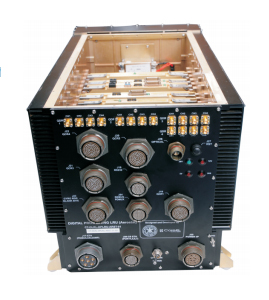
\includegraphics[width=0.3\paperwidth]{images/LRU.jpg}
            \caption{LRU}
            \label{fig:lru}
        \end{figure}
    \end{column}
    
    \begin{column}{0.45\paperwidth}
        \begin{figure}
            \centering
            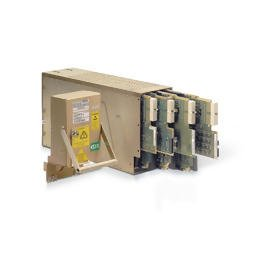
\includegraphics[width=0.3\paperwidth]{images/IMA.jpg}
            \caption{IMA}
            \label{fig:lru}
        \end{figure}
    \end{column}
  
  \end{columns}
  
\end{frame}


\begin{frame}[t]{Multicore based IMA} 
  
  \begin{center}
    \begin{mdframed}[style=yellowbox]
      {\small\textcolor{lightgray}{How to address} certification for multi-core based IMA \textcolor{lightgray}{platforms :
       current status and potential solutions}}
       \end{mdframed}
  \end{center}

    \begin{block}{Problématique}

    Peut-on atteindre une meilleure performance et le même niveau de déterminisme qu'un AMI mono-coeur sur un 
    AMI multi-coeurs ?

  \end{block}
 
\end{frame}

\section{Lists} 
\subsection{Itemize}

\begin{frame}{Itemize}
  \begin{itemize}
    \item Lorem ; \pause
    \item Ipsum ;
    \item Dolor : \pause
      \begin{itemize}
        \item Lorem,
        \item Ipsum ;
      \end{itemize}
    \item Sit amet.
  \end{itemize} 
\end{frame}


\subsection{Enumerate}
\begin{frame}{Enumerate}
\begin{columns}
  \begin{column}[l]{0.45\paperwidth}
      \begin{enumerate}
        \item Lorem ;
        \item<2-> Ipsum ;
        \item<2-> Dolor ;
        \item<2-> Sit amet.
      \end{enumerate}
  \end{column}

  \begin{column}[r]{0.45\paperwidth}
    Lorem ipsum dolor sit amet, consectetur adipiscing elit. Curabitur 
    ultricies, dui ac luctus pellentesque, nunc dui lobortis lorem, nec 
    porta mauris massa vel ante. Maecenas justo nisl, sodales quis 
    placerat nec, convallis mollis magna. Curabitur blandit elementum 
    elit et euismod. In et purus nisl, ac elementum orci.
  \end{column}
\end{columns}

\end{frame}

\section{Blocs}
%%%%%%%%%%%%%%%%%%%%%%%%%%%%%%%%%%%%%%%%%%%%%%%%%%%%%%%%%%%%%%%%%%%%%%%%%%%%%%%%%%%%%%%%%%%%%%%%%%%%%%%%%%%%%%%%%%%%%%%%
\begin{frame}{}
    \sectionframe{Blocks \\ \textit{Lorem ipsum dolor sit amet}}
\end{frame}

\begin{frame}{Block}
  \begin{block}{Aliquam quis eros}

    Aliquam quis eros nec risus mattis porttitor ac eget justo. 
    Aliquam lacinia condimentum tempus. Nulla metus magna, feugiat 
    id faucibus ut, commodo et justo. Aliquam tincidunt purus vitae 
    lacus dictum in placerat purus mollis. 

  \end{block}
\end{frame}

\begin{frame}{Example block}
  \begin{exampleblock}{Nulla cursus vehicula cursus}


    Nulla cursus vehicula cursus. Suspendisse ac enim eget purus 
    tincidunt eleifend et et purus. Suspendisse ultricies viverra 
    sodales. Proin non congue risus. Maecenas vel ornare sem. Ut 
    laoreet nibh tempor felis suscipit dignissim. Aliquam urna 
    eros, sagittis interdum ultrices sed, venenatis eu nisl.

  \end{exampleblock}
\end{frame}

\begin{frame}{Alert block}
  \begin{alertblock}{Quisque vehicula pretium arcu}

    Quisque vehicula pretium arcu, eget bibendum arcu iaculis sit amet. 
    Proin facilisis sollicitudin magna, et varius lorem euismod ornare. 
    Fusce lobortis dignissim tempor. Mauris augue tortor, elementum non 
    lobortis vel, interdum vitae augue.

  \end{alertblock}
\end{frame}

\end{document}
